\documentclass[11pt,a4paper,twoside,twocolumn]{article}

%--------------- Packages -------------------------------------------------
\usepackage{graphicx,parskip,times,amsfonts,amsmath}
\usepackage{jacobs-research-report}
\usepackage{eurosym}
\usepackage{natbib}
\usepackage{a4,a4wide}
\usepackage[latin1]{inputenc}
\usepackage[english]{babel}
\usepackage{amssymb,amsmath,amsfonts}
\usepackage{bibunits}
\usepackage{longtable}
\usepackage{bpchem}
%---------------------PDF-definitions--------------------------------------
\usepackage[pdftex,           %%% hyper-references for pdflatex
  hypertexnames=false,%       %%% needed for correct links to figures
  breaklinks=true,%           %%% break links if exceeding a single line
  colorlinks=true,%           %%% to underline links instead of boxing
  urlcolor=blue]{hyperref}    %%% blue instead of cyan URLS
%--------------------end-of-PDF-definitions-------------------------------
\usepackage{makeidx}
\makeindex

%--------------------User Definitions---------------------------------------- 
\hyphenation{Schlei-cher} \hyphenation{geo-me-try}
\newcommand{\C}{\mathbb{C}}
\newcommand{\R}{\mathbb{R}}
\usepackage{latexsym}
\newcommand{\bbbr}{\mathbb{R}}
\newcommand{\bbbn}{\mathbb {N}}
\newcommand{\bbbc}{\mathbb {C}}
\newcommand{\mycaption}[1]{\caption{#1}}
\renewcommand*{\cleardoublepage}{\clearpage\if@twoside \ifodd\c@page\else
    \hbox{}
    \if!\blankpagetext!\else
    \vfil \begin{center} \setlength{\fboxsep}{3mm}%
    \framebox{\blankpagetext}
    \end{center}\vfil\vfil \fi
    \newpage\if@twocolumn\hbox{}\newpage\fi\fi\fi}
\newcommand*{\resetpages}{\cleardoublepage\pagenumbering{arabic}}
\raggedbottom \pagenumbering{Roman}
\newenvironment{myitemize}{\begin{list}{-}{\labelwidth=0.2cm \leftmargin0.4cm
\labelsep0.2cm \rightmargin0cm \parsep0.5ex plus0.2ex minus0.1ex
\itemsep0ex
 plus0.2ex}}{\end{list}}

% new line after paragraph heading
\makeatletter
\newcommand\myparagraph{%
\@startsection{paragraph}{4}{\z@}%
{-3.25ex \@plus1ex \@minus.2ex}%
{.15ex \@plus.1ex \@minus.1ex}%
{\normalfont\normalsize\bfseries}}
\makeatother

\setlength{\parskip}{0pt plus 1pt}

%---------------------- Document ------------------------------------------------
\begin{document}
\def\Hchapter{\paragraph}
\def\bpchem{\BPChem}
%---------------- Path for images and pictures -------------------------------------
\graphicspath{{./MathTheoPhys/}{./Nano/}{./LifeSciences/}{./ESS/}{./EECS/}}


%----------------Title -------------------------------------------------------------
\title     {School of Engineering and Science \\
            Research Report 2007/2008} \shorttitle{RP 2007/2008}
\author    {Anke Allner}
\date      {2009 January}
\masterfile{SES--RR--2007/2008} 
\issue     {0} 
\revision {1} 
\version {2}{0}{05.01.09}{Test}
%-----------------------------------------------------------------------------------
\renewcommand{\refname}{\medbreak Publications\vadjust{\nobreak}}
\renewcommand{\bibname}{\medbreak Publications\vadjust{\nobreak}}
%-----------Table of Contents one column -------------------------------------------
\onecolumn
\shorttitle{Table of Contents} \tableofcontents \resetpages

%----------- Switch to two columns ----------------------------------------------------
\twocolumn

%------------ Intro Dean ---------------------------------------------------------------
\shorttitle{Introduction}
\section{Introduction}

With the outstanding financial investment of the Jacobs Foundation
in the Jacobs University on October 31, 2006 the future perspective
of the University and in particular the School of Engineering and
Science is on steady and forseeable grounds. This, and the advent of
the new president Professor Dr. Dr. h.c. mult. Joachim Treusch, who
formally took office by July 1, 2006, eventually resulted in a
reformulation of the key mission and the main research objectives of
the university. The main scientific activities of the School can be
considered to be perfectly consistent with the new objectives.

\subsection{The Mission}

The Jacobs University Bremen has been designed and developed as an
international research university using the anglo-saxon template,
and incorporating the European Bologna Process into its teaching
model. The main mission is to academically educate bright young
people, irrespective of their nationality, religion, sex, race and
financial conditions, in order to prepare them for future leading
roles in our globalized world. Thus, the University is designed to
provide significant contributions towards a peaceful, and
sustainable development of mankind. As a campus university where
students from more than 80 nations live and learn together in
colleges, intercultural understanding and collaboration in daily
life is trained as a byproduct of the university education.

\null
 Research and teaching are pursued on the same level and take
into account the requirements of practical life in enterprises and
industry. Interdiciplinarity constitutes the key concept. Research
at the Jacobs University Bremen aims at delivering key contributions
towards the main challenges of mankind, namely \\

\begin{myitemize}
\item   energy and materials,
\item  water and food,
\item   health,
\item "Bildung" and communication,
\item peace and conflict management.
\end{myitemize}


\null
 The School of Engineering and Science contributes with its
activities mainly towards the former three of these, although its
strong electrical engineering faculty addresses technological issues
that are closely related to the latter two.

The scientific objectives of Jacobs University concentrate in five
broad areas, namely \\

\begin{myitemize}
\item bio-geo-marine resources - from molecules towards technologies
\item  modelling of complex systems - computer simulation, visualisation, networks and management
\item changing societies, cultures, and institutions -  aspects of globalisation
\item   Asia and Europe - historical,
psychological and cultural perspectives
\item productive adult development \item "Bildung" and work
\end{myitemize}


\null
 The five research fields of the School of Engineering and
Science that have been emerging during the founding years contribute
towards the first two of these: Projects within "Information and
Communication Technologies" are directly related to the second
research area. Topics addressed by our "Life Sciences" and
"Geosciences and Astrophysics"  contribute to the first as well as
to the second area. "Nanoscience and Material Research" and
"Mathematics and Theoretical Physics" establish the scientific
backbones of the above. These provide important scientific tools and
the key methods for successfully tackling questions at the
interfaces between the conventional disciplines.

\null
The latter, namely science across disciplinary boarders is
indeed the outstanding - if not the main - trademark of research and
development,  and teaching at the  School of Engineering and
Science.


\subsection{Factual Development During the Founding Period}

\subsubsection{Students}
During the course of the past founding years, the School of
Engineering and Science has been showing remarkable growth, in
quantity as well as in quality. The number of undergraduate
students, starting in 2001 with 67 has now reached its preliminary
saturation at 381 students (Fig.~\ref{fig:students}). Basically this
is dictated by the number of college places and the fact that
according to planning 2/3 of the total number of students can be
admitted to programs of the School. There are now 12 undergraduate
programs of which 10 are formally accredited.


In 2004, for the first time a significant number (48) of graduate
students were admitted to the graduate programs of the School. Since
then, the number of graduate students has been growing to an
impressive total of 223 out of which 142 are PHD-students
(Fig.~\ref{fig:students}). By now, the school has successfully
established 7 graduate programs on the master's level.

\begin{figure}[ht]
  \begin{center}
   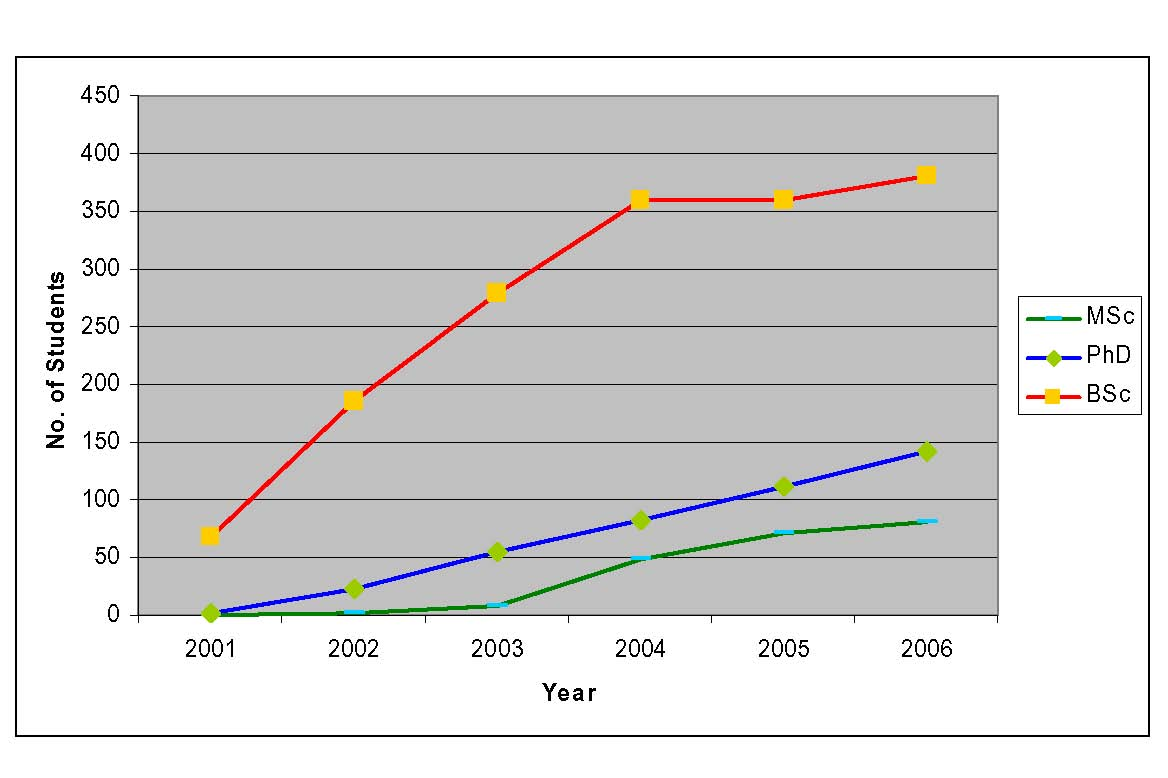
\includegraphics[width=\hsize]{Students.jpg}
   \end{center}
\caption{Temporal Development of Number of Students in the School of
Engineering and Science \label{fig:students}}
\end{figure}

\label{students}

\subsubsection{Publications}

During the founding period, the scientific output of the School,
measured in terms of the number of publications, has been growing
from initially 144 to 389 in 2006, after an intermediate decrease in
2004 which can be understood by having in mind that 2004 has been
the year during which the main research laboratories have been
planned and constructed (Fig.~\ref{fig:publications}). The last of
the laboratories (the EON laboratory) has been finished in 2005.

\begin{figure}[ht]
  \begin{center}
   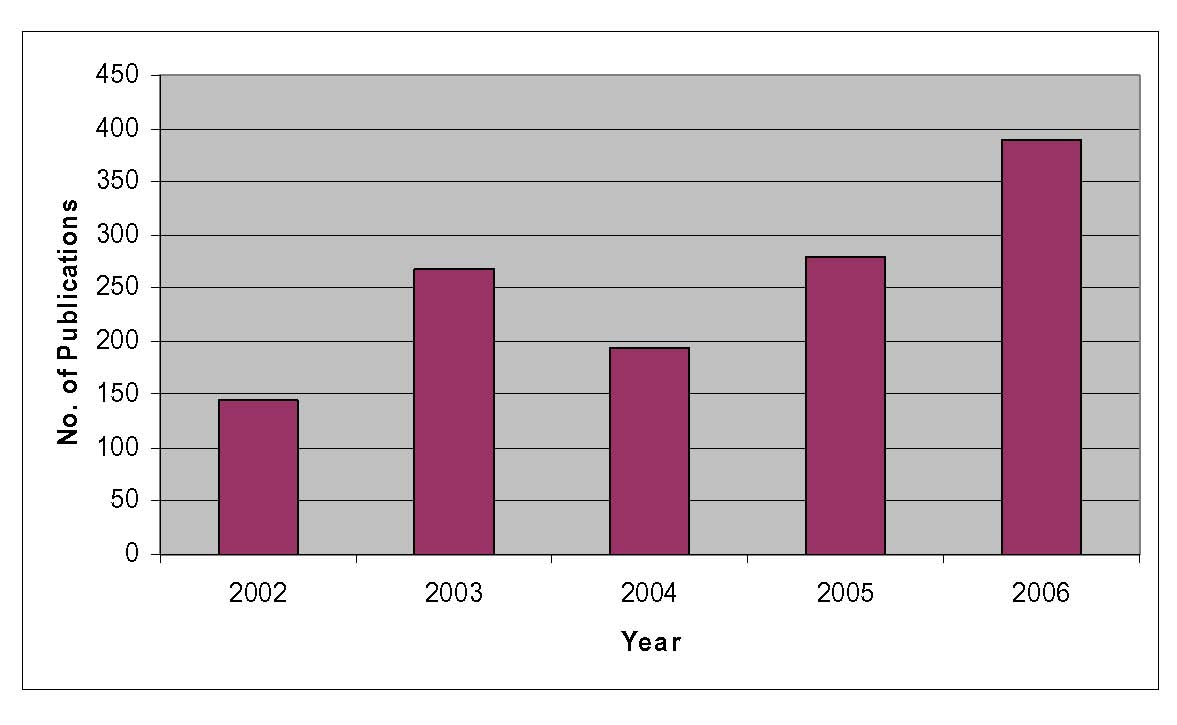
\includegraphics[width=\hsize]{Publications.jpg}
   \end{center}
 \caption{Number of Peer-reviewed Articles, Conference Proceedings, Articles in Encycl./Handbooks,
 Monographs/Books, Editor-ship, and Contribution in Ed. Volumes
 \label{fig:publications}}
\end{figure}


\subsubsection{Grants}
The development of third party funding is summarized in Figures
\ref{fig:grants1}, \ref{fig:grants2}. Revenues from Research grants
have reached a total of more than 4.000.000 EURO in 2006 which
implies an average revenue per professor of 82.000 EURO.

\begin{figure}[ht]
  \begin{center}
   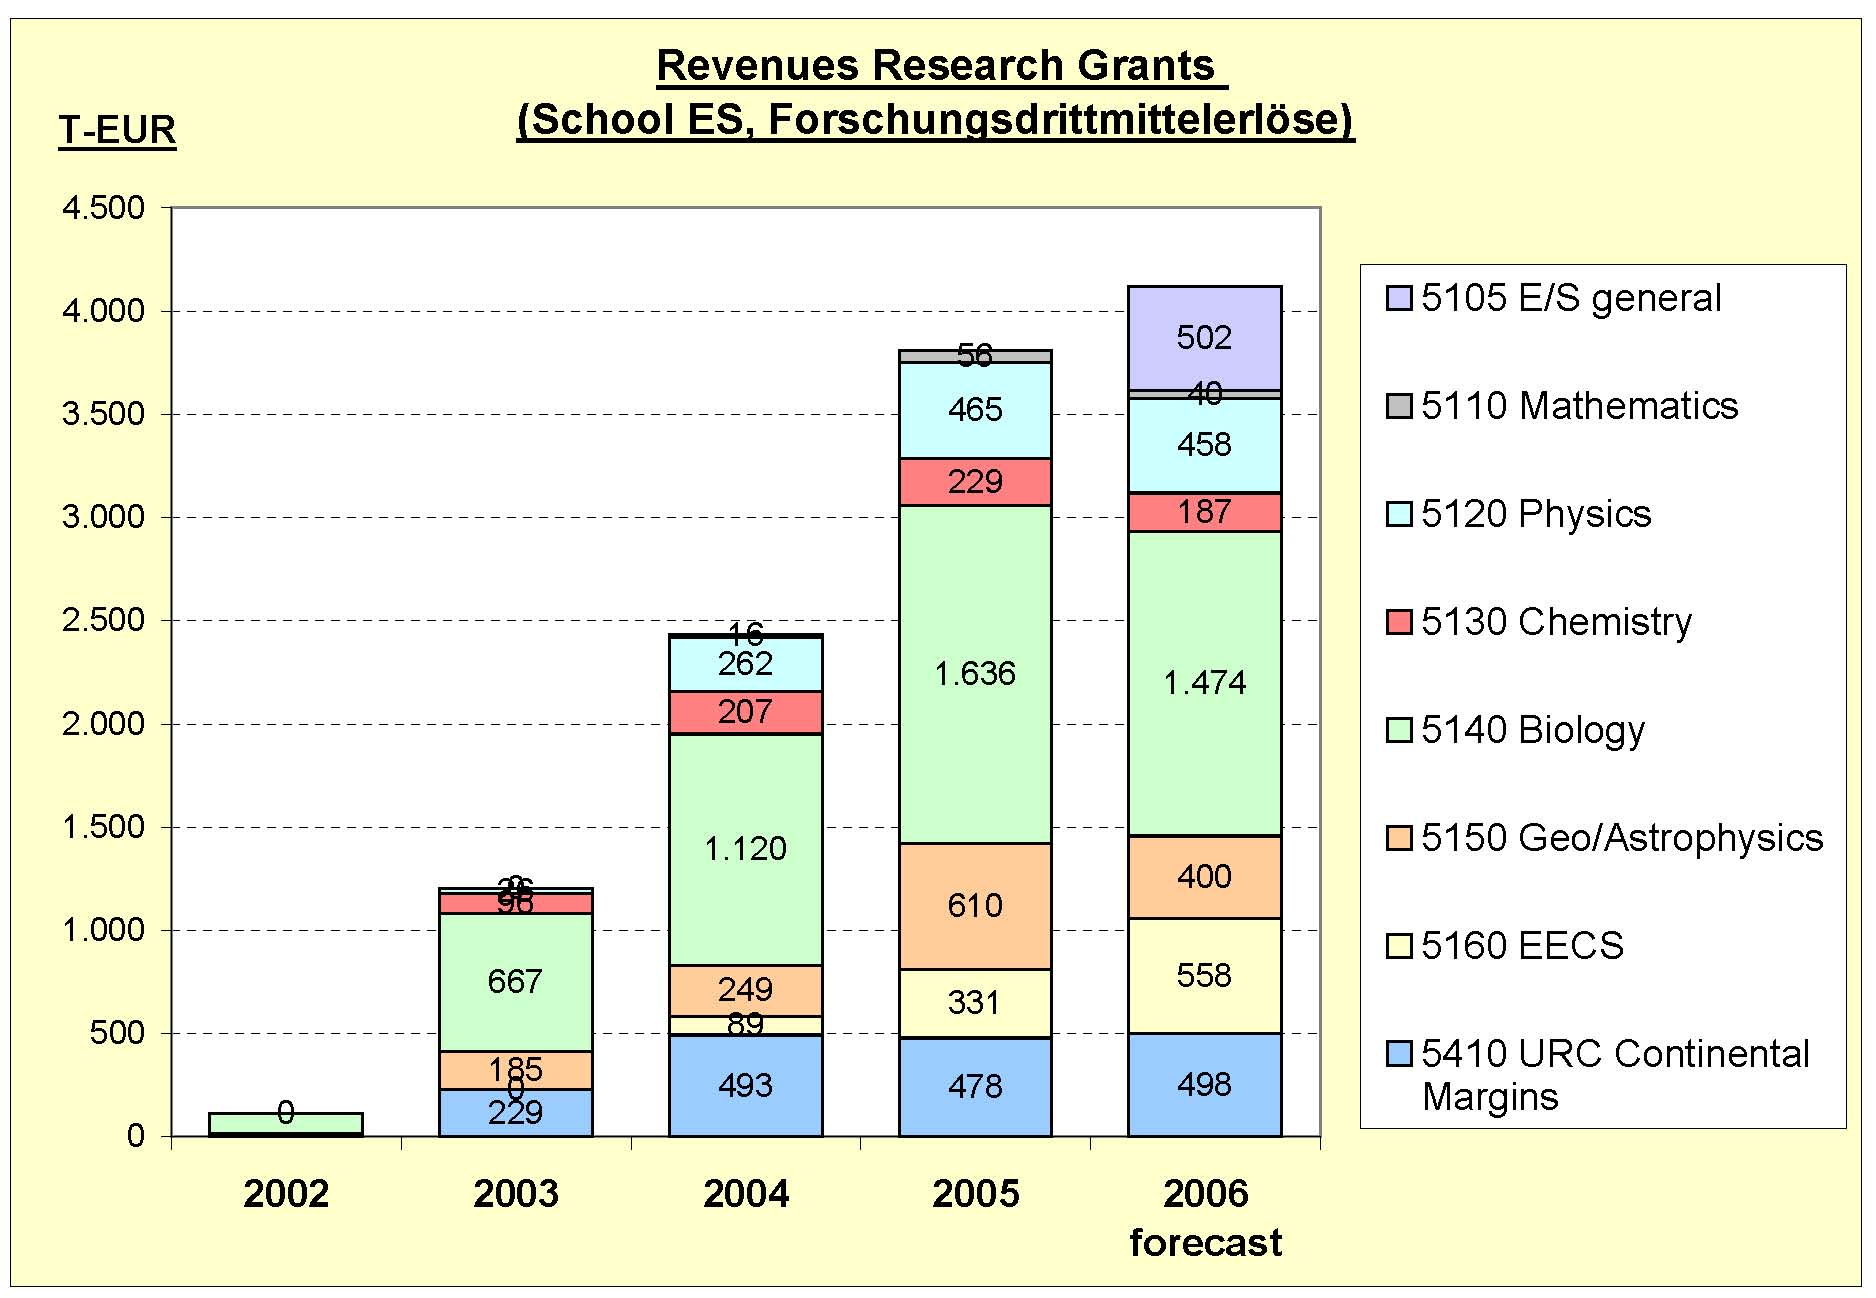
\includegraphics[width=\hsize]{SchoolESGrants-Charts1.jpg}

   \end{center}
 \caption{Research Grants  Revenue
 \label{fig:grants1}}
\end{figure}

\begin{figure}[ht]
  \begin{center}
   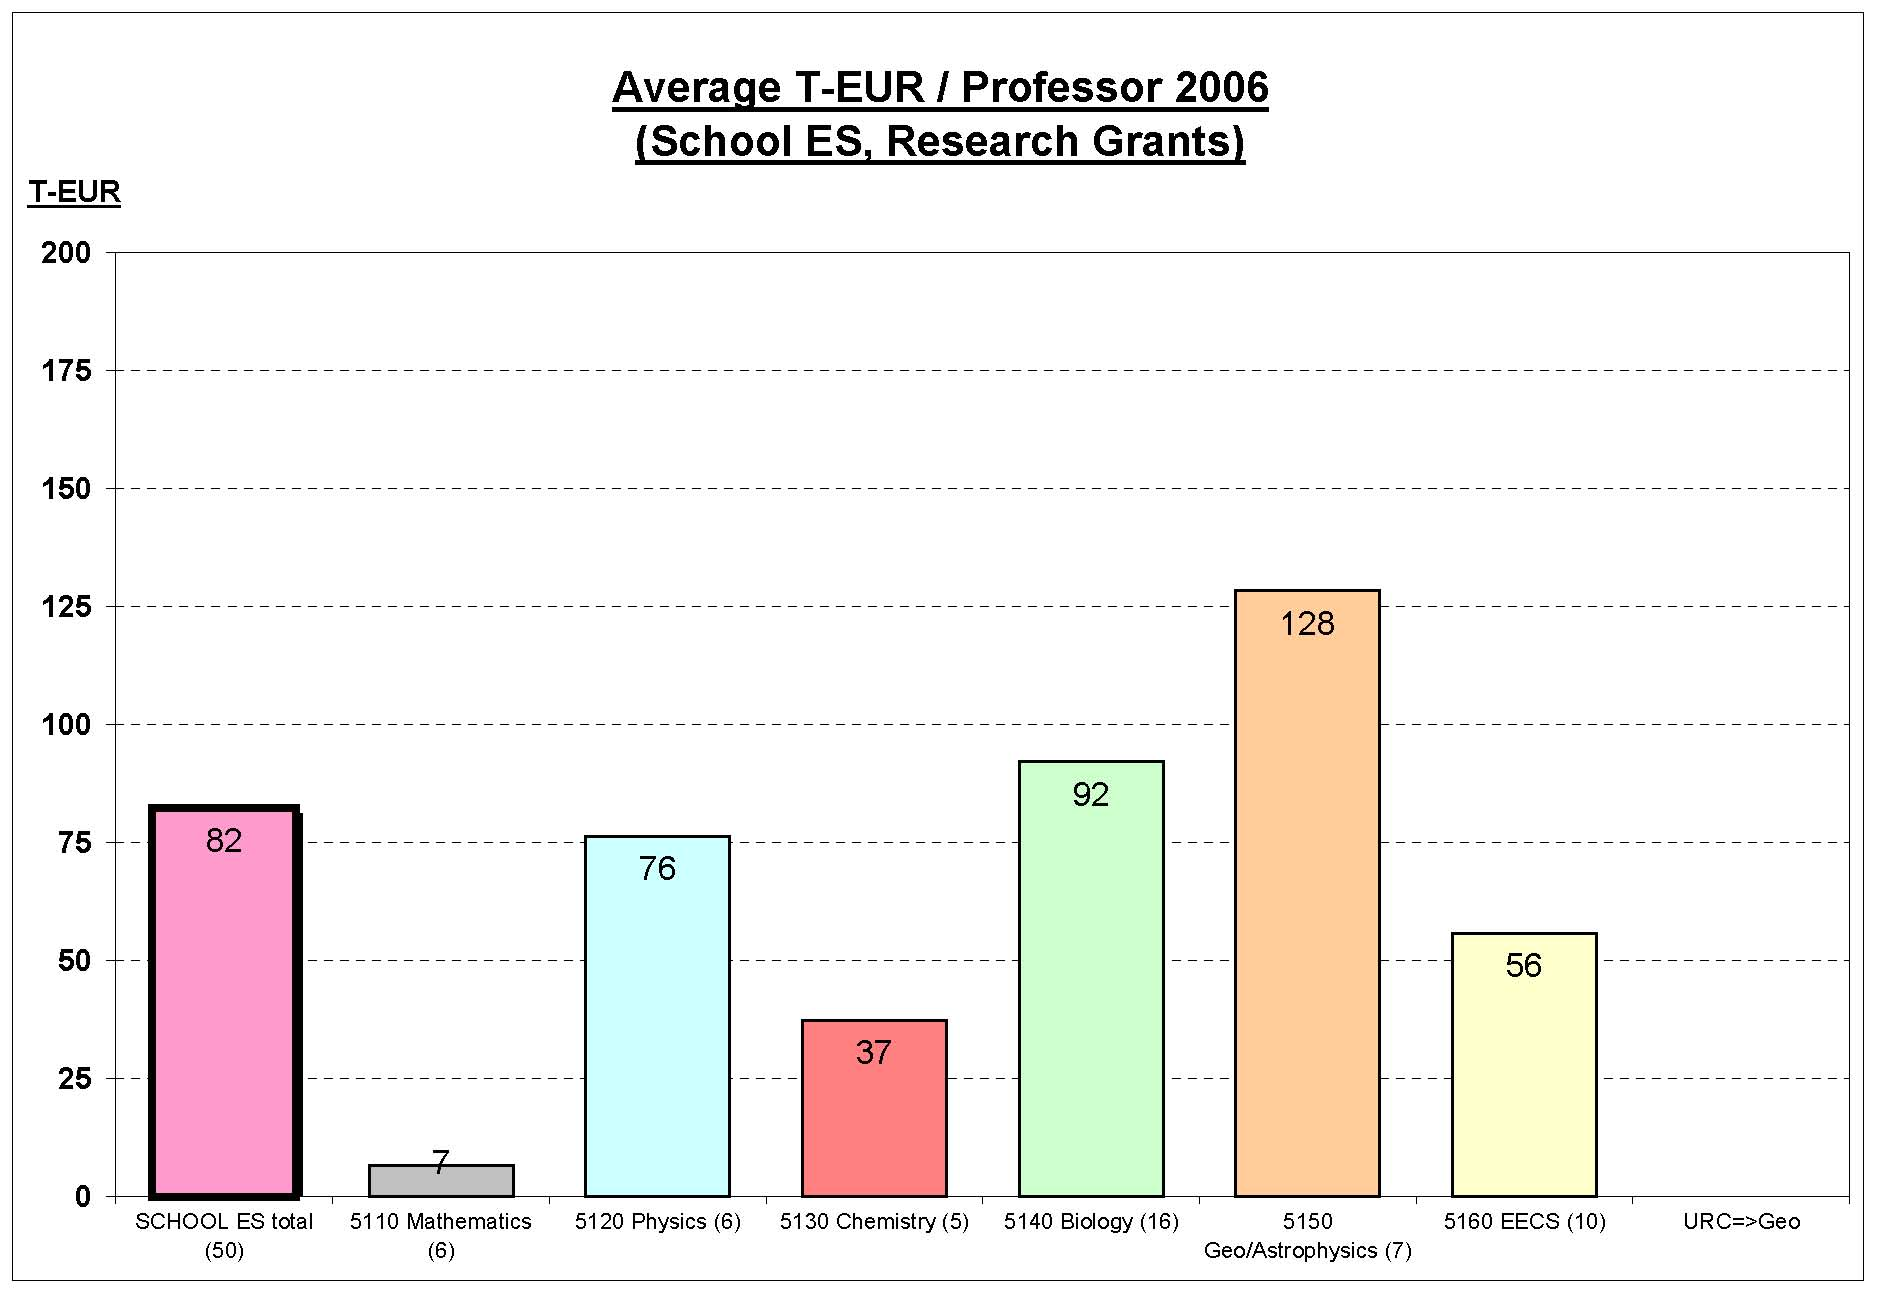
\includegraphics[width=\hsize]{SchoolESGrants-Charts2.jpg}
   \end{center}
 \caption{Research Grants Average T-EUR/Professor
 \label{fig:grants2}}
\end{figure}

\subsection{Personnel 2006} Presently, the school comprises in
total 64 professors out which 4 are adjunct professors, located at
the Alfred-Wegner-Institut in Bremerhaven and the Max-Planck-Insitut
f�r Marine Mikrobiologie in Bremen. Two distinguished professors and
6 university lecturers complete the faculty. In addition, 70
research associates, 5 research assistants, 26 technicians, 1
director and 7 assistants belong to the staff. In 2006, several new
faculty members have been hired.

\begin{myitemize}
 \item   Dr. Ulrich Kleinkath\"ofer, Associate Professor of
Theoretical Physics \item  Jon Wallace, PhD, Assistant Professor of
Electrical Engineering \item  Dr. Lars Linsen,  Associate Professor
of Computational Science and Computer Science \item   Dr. Bendick
Malehko, University Lecturer in Computer Science.
\end{myitemize}

In Mathematics, the visiting professors Prof. G. Litvinov and Prof.
Vladimir Tikhomirov, and Dr. Marc Comerford (research instructor)
left. They are replaced by \begin{myitemize} \item  Dr. Stefan Baier
(Visiting Lecturer for Mathematics) \item Kaivan Mallahi-Karai (PhD,
Visiting Lecturer for Mathematics) \item Dr. Alexei Belov (Visiting
Professor for Mathematics).
\end{myitemize}

The following members of the faculty have been promoted during 2006.
\begin{myitemize}
\item  Dr. Klaudia Brix from Associate to Full Professor
\item Dr. Albert Jeltsch from Associate to Full Professor
\item   Dr. Laurenz Thomsen from Associate to Full Professor
\item Marcus Br\"uggen Assistant to Associate
\item Claus C. Hilgetag, PhD from Assistant to Associate
\item Dr. Ulrich Schwaneberg from Assistant to Associate
\end{myitemize}

\null
Dr. Stefano Carpin, Assistant Professor of Computer Science,
has accepted an offer of an Assistant Professorship at University of
California, Merced, USA, starting on January 1, 2007.

\subsection{International Center for Transdisciplinary Science}
 The "International Center for Transdisciplinary Studies"
has been founded and started to operate. The center invites
internationally highly ranked scientists as fellows for periods of
several weeks, mostly during the summer break. The visiting
scientists are generally expected to participate in ongoing
scientific activities. In 2006, 46 scientists have been
participating, among them 39 from foreign countries:

\null Professor Dr. Roland Benz,   Universit\"at W\"urzburg, Germany
\\
Professor Dr.~Jan Bergstra,  University of Amsterdam, The Netherlands\\
Dr.~Andrey Bessonov, University of Sankt Petersburg, Russia\\
Dr.~S.M. Bezrukov,  National Institute of Health, Bethesda, USA\\
Dr. Georges Bouzerar,   Laboratoire Louis Nel, Grenoble, France\\
Dr. Henk Bruin  University of Surrey, United Kingdom\\
Professor Dr.~Mark Burgess,  University College Oslo, Norway\\
Professor Dr.~Val\'erie Cabuil,     Universit\'e Pierre et Marie
Curie, Paris, France\\
Dr.~Fabio Cavaliere, Universit\'a di Genova, Italy, Professor
Dr.~Shengbo Chen,      Institute of Geography and Natural
Resources, Beijing, China\\
Elizabeth Dan-Cohen,     University of California, Berkeley, USA\\
Professor Dr.~Gero Decher,      Institut Charles Sadron, Strasbourg,
France\\
Dr.~Martin Evans,        University of Edinburgh, United Kingdom\\
Dr.~Tom Fisher,      University of Cambridge, United Kingdom\\
Dr.~Claus F\"utterer,       Institut Curie, Paris, France\\
Professor Dr.~Mariano Grasselli,     Universidad Nacional de
Quilmes,
Argentina\\
Dr.~Giovanni Indiveri,       University of Lecce, Italy\\
Professor Dr.~Dieter J\"ager,      Emory University Atlanta, USA\\
Professor Dr.~Larry S. Liebovich,        Florida Atlantic
University,
USA\\
Professor Liviu Movileanu,      Syrakuse University, USA\\
Dr.~Sergei Nechaeev     CNRS Orsay, France\\
Professor Dr.~Catherine O'Neill,     Columbia University, USA\\
Dr.~Marieke Postma,     NIKHEF, Amsterdam, The Netherlands\\
Dr.~Enrico Ramirez-Ruiz,     Institute of Advanced Studies,
Princeton, USA\\
Professor Dr.~Helmut Ringsdorf,      Universit\"at Mainz, Germany\\
Dr.~Karin R\"omisch,       University of Cambridge, United Kingdom\\
Lucile Sassatelli,       ENSEA-ETIS, Cergy-Pontoise, France\\
Professor Dr.~J\"urgen Schnack,        Universit\"at Osnabr\"uck,
Germany\\
Professor Dr.~Gerhard Schwarz,       Biozentrum Basel, Switzerland\\
Professor Dr.~Vera Serganova,        University of California,
Berkeley, USA\\
Professor Dr.~Nobuo Shimamoto,      National Institute of Genetics,
Mishima, Japan\\
Professor Dr.~Canan Tari,        Izmir Institute of Technology,
Turkey\\
Professor Dr.~Alexander Tikhomirov,  Yaroslavl State Pedagogical
University, Russia\\
Dr.~Andrew Travers,      Medical Research Council, Cambridge, United
Kingdom\\
Dr.~Martin Weigt,        ISI Foundation, Torino, Italy\\
Professor Dr.~James Whisstock,      Monash University, Victoria,
Australia\\
Dr.~Wojtek Zakrzewski,   University of Durham, United Kingdom\\
Dr.~Michael Zaks,    Humboldt-Universit\"at Berlin, Germany\\
Professor Dr.~Gregg Zuckerman,   Yale University, USA.

\subsection{Workshops and Summer Schools 2006}

During the year, several international research workshops have been
organized on the campus by members of the faculty.

\begin{myitemize}
\item
From October 19-22, 2006 the International Workshop on Astrobiology
took place at IUB, organized by Professor Michael Bau.  Focus of the
workshop were Banded Iron Formations (BIFs), that developed between
two and four billion years ago in the precambrian era.  The workshop
aimed at providing an overview on current ideas on the formation and
preservation of Precambrian BIF, on the use of BIF as proxies for
Precambrian seawater, on differences between Early Precambrian BIF
and younger ironstones and hydrogenetic Fe(-Mn) precipitates, and on
experimental set-ups to simulate BIF-related processes in Early
Precambrian environments.

\item
A workshop for young scientists is offered biannually by the DFG
Schwerpunktprogramm SPP1170 (priority program) ''Directed Evolution
to Optimize and Understand Molecular Biocatalysts''. This year's
workshop  took place from July 30 until August 1 on the IUB campus,
organized by Professor Ulrich Schwaneberg. 70 scientists from the 17
DFG institutions participate in the program. They presented and
discussed the research and its influence on applications with
representatives from companies.


\item
From July 28 until August 5, a Summer School for students and
postdocs  took place. Focus of the more than 50 lectures and
workshops has been on recent research perspectives in biosensing and
its application. 70 participants from 14 Nations met on IUB campus.
This summer school  covered applications of membrane channels in
molecular biology and biotechnology. In addition, it informed on the
underlying physics and will present recent advances in microfluidics
and nanoelectronics. The fourth IUB Summer School has been organized
by Dr. Mathias Winterhalter, Professor of Biophysics at IUB. The
Summer School offered students and postdocs the opportunity to
advance their understanding of biosensing, present their research
and build networks.


\item In June 2006, the 10th International RoboCup has been organized
in Bremen. More than 400 teams and 2500 participants from 36
countries participated and competed in three main categories: the
robot soccer competition, the robot rescue competition (coordinated
by Prof. A. Birk), and the RoboCupJunior for educational purposes.
On June 18, the finals of the Robot Rescue League took place in the
Congress Center Bremen. IUB teams participated in both competitions
the ''Rescue Robot League�� and the ''Virtual Robot Competition��.
The team led by Andreas Birk, Professor of Electrical Engineering
and Computer Science, reached the finals of the Robot League and won
the Innovation Award, a student team led by Stefano Carpin,
Professor of Computer Science came in second place in the Virtual
Robot Competition.

\item
From the 16th to 20th of January, IUB  hosted the international
"HERMES Graduate Training and Job Fair". More than 30 Master's and
PhD students working at HERMES partner institutions all over Europe
participated. The fair offered students and Postdocs the opportunity
to advance their understanding in aspects of marine science outside
their own fields and to present and discuss their own research (Jan
10, 2006). The HERMES (Hotspot Ecosystem Research on the Margins of
European Seas) Program, funded by the European Commission, was begun
to gain better understanding of life in depths of between 200 and
2000 meters and deeper.

\end{myitemize}


\subsection{Research Highlights}

Researchers of the School of Engineering and Science have been
contributing towards the international scientific progress with
several important discoveries that have been published in the most
prestigious international journals.

\begin{myitemize}
\item
Albert Jeltsch, IUB Professor of Biochemistry, and his co-workers
from IUB, the Institute of Biochemistry of the University of
Giessen, and the Medical Research Council of Cambridge University
(UK) for the first time successfully used genetically engineered
proteins to deactivate Herpes viruses in human cell lines. The study
is published in the November 2006 issue of Nucleic Acids Research

\item
Stefan Tautz, IUB Professor of Physics, and his group for the first
time managed to detect a much larger delocalization of electrons in
an organic monolayer semiconductor deposited on a metallic substrate
than ever detected in an insulated organic semiconductor. The
results, which were published in Nature 444, p. 350 - 353, on
November 16, 2006, allow insights into basic mechanisms of electron
transport within organic materials and their interfaces with
metallic surfaces. Moreover, the results may be of relevance for the
development of new hybrid materials with interesting new electronic
properties regarding future application.



\item
On the 68th cruise of the German research vessel METEOR an
international team of scientists under the lead of Andrea
Koschinsky, Professor of Geosciences at IUB, registered 407
$^{\circ}$ C at a hydrothermal vent as the highest temperature on
record measured at the ocean bottom (May 22, 2006).  Using a special
temperature sensor operated by a deep-sea robot the scientists
registered the record temperature in 3000m water depth at a
so-called ''black smoker'', a hydrothermal deep-sea vent with a
characteristic particle plume in the discharge water. Moreover, the
boiling fluids emitted by the vent were filmed. The super-hot vent
was discovered at 5 $^{\circ}$ S at the Mid-Atlantic Ridge, where
the African and the South American continental plates drift apart 4
cm per year, causing increased volcanic activity. Normally the
temperature of the circulating seawater cooling the volcanoes
emerging in this area does not exceed a maximum of about 350
$^{\circ}$ C when welling out of the sea floor. Maximum deep-sea
water temperatures up to 402 $^{\circ}$C so far have only been
observed in the Pacific.




\item
Stephan Rosswog, Professor of Astrophysics at IUB, and Daniel Price,
Postdoc at the University of Exeter, for the first time were able to
demonstrate in supercomputer simulation of a neutron star merger
that a collision of these super dense cosmic objects create magnetic
fields a quadrillion (10$^{15}$) times stronger than the magnetic
field of the earth. The simulation results are published in the
current online express issue of Science ("Producing ultra-strong
magnetic fields in magnetized neutron star mergers", 30 MARCH 2006).

\item
Claus Hilgetag, Professor of Neuroscience at IUB, and his colleague
Helen Barbas, Professor of Health Sciences at Boston University,
found new answers to one of the oldest questions in neuroscience:
How do the characteristic folds of the primate brain cortex form?
The results of an extensive analysis of neuroanatomic data are
published as the cover story in the latest issue of PLoS
Computational Biology ("Role of Mechanical Factors in the Morphology
of the Primate Cerebral Cortex", Volume 2, Issue 3, MARCH 2006,
www.ploscompbiol.org).  By analyzing quantitative data collected in
the lab of Helen Barbas over a period of two decades, Claus Hilgetag
for the first time was able to provide empirical evidence for the
hypothesis that the characteristic folds of the primate brain are
mainly formed by mechanical forces of fiber tension.


\end{myitemize}


\subsection{Noteworthy}
\begin{myitemize}
\item
On November 15, 2006, the association ''Unifreunde e. V.�� awarded
the Ernst A. C. Lange Prize for the joint research project ''New
display technology for mobile applications�� of IUB and University
of Bremen. The award, which is endowed with 5000 euros prize money,
acknowledges innovative co-operational research between scientists
of the two Bremen universities in the fields of Mathematics, Natural
and Technical Sciences. The two laureates 2006 are the two Bremen
scientists Dietmar Knipp, Professor of Electrical Engineering at
IUB, and Wolfgang Benecke, Professor of Physics, Electronics and
Information Technology at University of Bremen. The aim of their
joint research project is the development of a new type of
projection display for mobile application such as laptop computers,
mobile phones, and digital cameras.


\item Researchers from all over Germany were taking part in the Science
Festival "Highlights of Physics" from 6-10 November 2006 in Bremen.
Under the motto of "WaveWorlds" scientists gave an introduction into
wave phenomena in water, light and sound through series of talks,
live experiments and science shows.  IUB was involved in the
organization and preparation of this event. Faculty and staff
contributed in particular to the big opening show, the exhibition,
and the physics competition for pupils.

\item
In October the research network International Research Consortium on
Continental Margins (IRCCM) under IUB's lead started a new research
project on biomonitoring of cold water coral reefs in the vicinity
of oil exploration sites. The aim of the 1.2 million euro project
financed by the Norwegian company Statoil is to develop new
monitoring and ecosystem modelling approaches for risk assessment in
the off-shore industry.  Research site is the Tisler cold water
coral reef in the Skagerrak, which was placed under environmental
protection by the Norwegian government in 2003. As part of the EU
HERMES project (Hotspot Ecosystem Research on the Margins of
European Seas) it is managed by HERMES partner Tj\"arn\"o Marine
Biological Laboratory (TMBL) and will host IUB's second deep-sea
online observatory.


\item
On April 23, 2006, IUB's RoboCup team managed another international
tournament victory at the US Open Robot Rescue League in Atlanta,
prevailing against the other competing institutions only two weeks
after their success at the Dutch Open in Eindhoven (Apr 25,2006).
The ten contesting teams in Atlanta included such renowned
institutions as the Georgia Institute of Technology and Carnegie
Mellon University, which demonstrated with their impressive
investments into their teams the importance of research on search
and rescue robots in the US. Georgia Tech had two teams within the
competition, one of them using the best mobile research platform
that is currently available on the market. A team from Carnegie
Mellon University had even six robots running including a high-end
commercial platform for search and rescue missions.

\item
Informatics Year is being organised in conjunction with the Science
in Dialogue initiative and the Gesellschaft f�r Informatik (GI) as
well as with numerous partners in the fields of science, industry
and culture. The idea behind this Science Year was to familiarise a
broader public with the contents, processes and practical
applications of science and to do so in an informative, exciting and
entertaining way. IUB was involved in exhibitions, the Symposium on
Artificial Intelligence and various other activities.

\end{myitemize}
\ \ \\
\ \ \\

Bremen, January 2007


\begin{figure}[ht]
     
\includegraphics[width=4cm]{DeanSig}
 \end{figure}



Bernhard Kramer
 
\cleardoublepage % Each chapter starts on a right page 
%------------ EECS ---------------------------------------------------------------------
\input{./LifeSciences/Introxxx}
\begin{bibunit}[hplain]
\input{./LifeSciences/xxx}
\input{./LifeSciences/xxx_bib}
\end{bibunit}
\begin{bibunit}[hplain]
\input{./LifeSciences/xxx}
\input{./LifeSciences/xxx_bib}
\end{bibunit}


\end {document}

 
